\documentclass[11pt]{article}
\usepackage[T1]{fontenc}
\usepackage[utf8]{inputenc}
\usepackage{lmodern}
\usepackage[margin=1in]{geometry}
\usepackage{amsmath,amssymb,amsthm,mathtools}
\usepackage{booktabs,array,graphicx,enumitem}
\usepackage{microtype}
\usepackage{xcolor}
\usepackage[colorlinks=true,linkcolor=blue!50!black,citecolor=blue!50!black,urlcolor=blue!50!black]{hyperref}
\usepackage{url}

\theoremstyle{plain}
\newtheorem{theorem}{Theorem}[section]
\newtheorem{proposition}[theorem]{Proposition}
\newtheorem{lemma}[theorem]{Lemma}
\newtheorem{corollary}[theorem]{Corollary}
\theoremstyle{definition}
\newtheorem{example}[theorem]{Example}
\newtheorem{remark}[theorem]{Remark}
\numberwithin{equation}{section}

\newcommand{\R}{\mathbb R}
\newcommand{\eps}{\varepsilon}
\newcommand{\compatible}{\mathcal C}
\newcommand{\outerset}{\mathcal O}
\newcommand{\gmin}{g_{\min}}
\newcommand{\Bseq}{B_{\mathrm{seq}}}
\DeclareUrlCommand\lean{\urlstyle{tt}}
\newcommand{\Lean}{\textsf{L}}   % evidence tag: statement compiled in Lean
\newcommand{\Conv}{\textsf{C}}   % evidence tag: conventional proof in this paper
\setlength{\emergencystretch}{2em}
\setlength{\belowcaptionskip}{6pt}

\title{When dilution resolves a low sandwich-immunoassay signal:\\
robust certificates and the limits of spike controls}
\author{}
\date{}

\begin{document}
\maketitle
\vspace{-3em}
\begin{abstract}
A low sandwich-immunoassay signal can mean little analyte, or so much analyte that
capture and detection reagents are spread over different molecules (the high-dose
hook effect). We ask what a second reading of a diluted aliquot certifies in a
finite-reagent, independent-site equilibrium model when capacities, affinities,
dilution factor, gain drift and native availability are known only to within
intervals. The noise-free ambiguity is described exactly: the response is strictly
unimodal, every sub-maximal signal has exactly two preimages (exchanged by an
involution for symmetric sites), and the diluted-to-neat ratio is strictly
increasing. We then prove robust two-reading certificates: for near-unit
parameters, dilution in $[9,11]$ and $5\%$ gain drift, the diluted-minus-neat source
contrast is nonpositive for accessible concentration at most $0.4$ and at least
$0.04$ on $[20,100]$; a general-box theorem gives analogous margins when capacities
exceed dissociation constants a hundredfold, for unequal capacities, and up to
$10^4$ with an explicit $1/U$ law. Each continuum inequality reduces to eight
positive Bernstein coefficients. We derive error budgets from precision profiles, a
reduction of relative error to gain drift, conclusions without a binary promise
and extensions to availability drift and incomplete equilibration, with a kinetic
theorem giving a sufficient incubation time. Exact indistinguishability results
show what a neat reading, accessible spikes and finite dilution panels cannot
certify. For sequential assays, ideal washing gives a monotone saturating response,
any fixed carry-over restores the high-dose tail, and a finite-range wash
specification is given. The source inequalities, decisions, certificates and
obstructions are verified in Lean~4; the structural and kinetic theorems have
conventional proofs. These are conditional certificates, not clinical
performance claims.
\end{abstract}

\section{Introduction}\label{sec:intro}

\subsection{The inference problem}
In a two-site (sandwich) immunoassay an analyte is recognised by a capture reagent
and by a labelled detection reagent, and the measured signal reports analyte that
carries both \cite{miles1968,wild2013}. When capture and detection reagents meet
the specimen simultaneously, the response is not monotone. At sufficiently high
concentration the finite reagent supplies are distributed over different analyte
molecules, doubly occupied complexes become rare, and the signal falls back
towards the blank. This high-dose hook (or prozone) effect has been analysed
experimentally and theoretically for decades
\cite{rodbardweiss1973,rodbard1978a,rodbard1978b,ryall1982,fernando1992a}, remains a recognised source
of falsely low results in clinical chemistry
\cite{selby1999,tate2004,sturgeon2011,hoofnagle2009}, and belongs to the wider
family of bell-shaped three-body binding responses \cite{douglass2013,roy2017}.

The standard remedy is dilution: if a diluted aliquot reads \emph{higher} than
the neat specimen, the neat reading was on the descending limb
\cite{butch2000,jacobs2015}, and dilution linearity with an explicit hook check is
part of ligand-binding assay validation \cite{desilva2003,ichm10}.
Upfront dilution has improved a ferritin workflow \cite{wu2018}; reaction-rate
monitoring and real-time kinetics flag antigen excess or extend the usable range
\cite{hoffman1984,rey2017,sathishkumar2020}; but dilution also degrades accuracy when the specimen matrix departs from the
validated one \cite{hunsaker2024}, and in lateral-flow formats even the control
line can depend on concentration \cite{ross2020}. The practical question is
therefore not whether dilution can help. It is what, exactly, a neat/diluted pair
of raw readings certifies when nothing about the assay is known exactly:
reagent capacities and affinities lie in calibration intervals, a nominal tenfold
dilution is really a factor somewhere in $[9,11]$, the instrument gain drifts
between the two readings, readings carry error, and only a fraction of the native
analyte may be recognisable by the antibody pair.

\subsection{Contributions}
We treat this as a problem of robust inference under a mass-balance source model
with interval-valued calibration, in the spirit of partial identification
\cite{manski2003}: a conclusion is admissible only if it holds for every state of
the world compatible with the declared assumptions. The contributions are as follows.

\begin{enumerate}[leftmargin=2em,itemsep=2pt]
\item \emph{Exact structure of the ambiguity} (Section~\ref{sec:structure}). For
every parameter choice the equilibrium response $B(u)$ is strictly unimodal, its
logarithmic slope decreases strictly from $1$ to $-1$, every sub-maximal level has
exactly two preimages, and the diluted-to-neat ratio $B(u/d)/B(u)$ increases
strictly from $1/d$ to $d$. When the two sites have equal $C+K=D+J=S$ the two
preimages are exchanged by $u\mapsto S^2/u$. Hence a neat reading is ambiguous for
every assay in the model class, and the sign of the dilution contrast has a single
crossover concentration.
\item \emph{A robust two-reading certificate} (Section~\ref{sec:certificate}). We
prove uniform source margins over full calibration boxes by retaining the reagent
product shared by both readings and reducing a two-variable polynomial inequality to
eight positive Bernstein coefficients. A general-box theorem covers arbitrary
positive calibration intervals; worked instances include a near-unit box, a
high-capacity regime with $C/K\approx100$, unequal capture and detector capacities,
and ranges up to $10^4$ with an explicit $7371/(8000\,U)$ law.
\item \emph{From margins to decisions} (Section~\ref{sec:decisions}). Additive-error
budgets, one-sided exclusions that need no low-or-high promise, a sound outer
enclosure of the compatible concentrations, a bridge from a precision profile to a
deterministic error allowance with stated coverage, and an exact reduction of
bounded relative error to gain drift.
\item \emph{Exact limits} (Section~\ref{sec:limits}). Three observational
equivalences show what cannot be certified: a neat reading alone; native
concentration from fully accessible spikes when native masking persists; and
exclusion of an unbounded high tail by any finite dilution panel with nonzero
error. The sufficient operating ceiling and the obstruction both scale as $1/\eps$.
\item \emph{Departures from the ideal protocol} (Section~\ref{sec:physical}).
Availability that changes on dilution is an effective change of dilution factor; a
calibrated attenuation bound suffices for incompletely equilibrated readings; and
for well-mixed mass-action kinetics started unbound we prove the attenuation bound
$(1-e^{-\lambda_Ct})(1-e^{-\lambda_Dt})$ with explicit rates, which converts rate
constants into a sufficient incubation time.
\item \emph{Sequential assays} (Section~\ref{sec:sequential}). With ideal washing
the response is strictly increasing and approaches a positive plateau at an
explicit rate; with any carry-over fraction $\lambda>0$ it decays like
$CD/(\lambda u)$; and a wash specification $\lambda_{\max}U\le D_{\min}(\beta^{-1}-1)$
preserves a fraction $\beta$ of the ideal signal on a finite range.
\end{enumerate}

\subsection{Evidence levels and scope}
Statements are tagged \Lean{} when the displayed statement has been compiled in
Lean~4 with mathlib \cite{demoura2021,mathlib2020} under the strict regime described
in Section~\ref{sec:verification} (Table~\ref{tab:formal} lists the declarations),
and \Conv{} when the proof is the conventional one given here. Numerical
illustrations are labelled as such and carry no claim. All worked numbers are
replayed by a script distributed with the source.

We do not claim priority for dilution protocols, kinetic rescue, mass-action models
of the hook effect, or partial identification; the closest modelling work
\cite{rodbard1978b,fernando1992a,fernando1992b,douglass2013,qian2003} derives and
fits response curves, whereas the present paper asks which decisions remain valid
uniformly over calibration uncertainty and proves them. We do not establish a
clinically superior protocol. The model is homogeneous, noncooperative and
two-site; immobilised reagents, multivalency, cooperative binding \cite{roy2017},
transport in lateral-flow strips \cite{qian2003,ross2020} and matrix effects are
outside it, and the assumptions are part of every result.

\section{Source, protocol and observation model}\label{sec:model}

\subsection{Finite-reagent equilibrium}
Let $x\ge0$ be the total native analyte concentration and $u=\rho x$ the
concentration that is accessible to both antibodies, where $\rho\in(0,1]$ is an
availability fraction. The analyte has two distinct, independent binding sites.
The effective capture and detector binding-site capacities are $C,D>0$ and the
site dissociation constants are $K,J>0$; all concentrations refer to the final
reaction volume. Writing $p,q\in(0,1)$ for the occupied fractions of the two sites
on accessible analyte, conservation of each reagent gives
\begin{equation}\label{eq:balance}
 C=up+\frac{Kp}{1-p},\qquad D=uq+\frac{Jq}{1-q},\qquad B(u)=upq .
\end{equation}
The four analyte species $u(1-p)(1-q)$, $up(1-q)$, $u(1-p)q$, $upq$ are
nonnegative and sum to $u$; the free reagents are $C_f=Kp/(1-p)$ and
$D_f=Jq/(1-q)$. The identities $C_f(1-p)=Kp$ and $D_f(1-q)=Jq$ are the four
mass-action equilibria with the same site constant whether or not the other site is
occupied; this is the independent-site assumption. Thus \eqref{eq:balance} is a
mass-balance source and not a fitted hook-shaped curve. The signal-generating
species is the doubly occupied complex $B(u)$. The capture equation is a quadratic
for $w=up$, namely $(C-w)(u-w)=Kw$, whose physical root gives the numerically stable
expression
\begin{equation}\label{eq:root}
 p(u;C,K)=\frac{2C}{u+C+K+\sqrt{\smash[b]{(u-C)^2+2K(u+C)+K^2}}} ,
\end{equation}
used for illustrations only. The proofs use \eqref{eq:balance} directly.

\begin{lemma}[Physical root and envelopes; \Lean]\label{lem:source}
For $u\ge0$ and $C,K>0$ the capture equation in \eqref{eq:balance} has exactly one
root $p\in(0,1)$, and
\begin{equation}\label{eq:pbounds}
 \frac{C}{u+K+C}\le p\le\frac{C}{u+K},\qquad up\le C .
\end{equation}
The same holds for the detector site, and therefore
\begin{equation}\label{eq:envelopes}
 \frac{CDu}{(u+K+C)(u+J+D)}\le B(u)\le\frac{CDu}{(u+K)(u+J)},
 \qquad B(u)\le u,\qquad uB(u)\le CD .
\end{equation}
\end{lemma}
\begin{proof}
The polynomial $(C-up)(1-p)-Kp$ is positive at $p=0$ and negative at $p=1$, so a
root exists; the right side of the capture equation is strictly increasing in $p$,
so it is unique. Mass balance gives $C\ge(u+K)p$, and $K/(1-p)=K+C_f\le K+C$ gives
$C\le(u+K+C)p$. Multiplying the two sites' bounds gives the envelopes, $p,q<1$
gives $B\le u$, and $up\le C$, $uq\le D$ give $uB\le CD$.
\end{proof}

The envelopes already exhibit both tails. For small $u$ the response is linear,
$B(u)\sim\alpha u$ with $\alpha=CD/((C+K)(D+J))$; for large $u$,
\begin{equation}\label{eq:tailexp}
 B(u)=\frac{CD}{u}-\frac{CD(K+J)}{u^2}+O(u^{-3}),
\end{equation}
because each limited reagent population is spread over many analyte molecules.
A monotone Hill curve has no such second tail; conversely, \eqref{eq:balance} is one
architecture and not every sandwich assay.

\subsection{Protocol, calibration box and observations}
Two matched reactions are prepared. The specimen is diluted by a factor $d$
\emph{before} fresh reagents are added, so that both reactions have the same
$C,D,K,J$ in the same final volume. Diluting an already assembled reaction changes
$C$ and $D$ as well and is a different experiment. The blank-corrected raw readings
and their contrast are
\begin{equation}\label{eq:obs}
 Y_1=gB(u)+e_1,\qquad Y_d=grB(u/d)+e_d,\qquad Z=Y_d-Y_1 ,
\end{equation}
with common gain $g\ge\gmin>0$, relative gain $r$ between the readings, and
additive errors with $|e_1|,|e_d|\le\eps$. The error allowance is one simultaneous
deterministic bound that includes every admitted additive contribution once; no
distribution or independence is assumed (Section~\ref{sec:precision} connects it to
a precision profile). The running example is the \emph{near-unit box}
\begin{equation}\label{eq:box}
 C,D,K,J\in[\tfrac9{10},\tfrac{11}{10}],\qquad d\in[9,11],\qquad
 r\in[\tfrac{19}{20},\tfrac{21}{20}],\qquad \rho\in[\tfrac45,1].
\end{equation}
The source contrast is $\Delta(u)=rB(u/d)-B(u)$, so that $Z=g\Delta(u)+e_d-e_1$.

\paragraph{Units.} Concentrations are expressed relative to a chosen scale $c_0$
($x=x_{\rm phys}/c_0$, and likewise for $C,D,K,J$); raw signals use a separate
scale. A change of units cannot force the four ratios among $C,D,K,J$ to be near
one, so \eqref{eq:box} is a genuine restriction. Section~\ref{sec:general} removes it.

\paragraph{Availability.} The factor $\rho$ is a two-population reduction:
fully recognised analyte at concentration $u$, plus analyte invisible to the pair.
Partially masked analyte that still consumes one reagent acts as a competitor and
needs a larger model.

\section{The exact structure of the ambiguity}\label{sec:structure}

Before adding uncertainty we describe the noise-free source completely. Let
$E_C(u)=-u\,p'(u)/p(u)$ be the elasticity of the capture occupancy, $E_D$ the
detector analogue, and $L_B=\mathrm d\log B/\mathrm d\log u$.

\begin{figure}[t]
\centering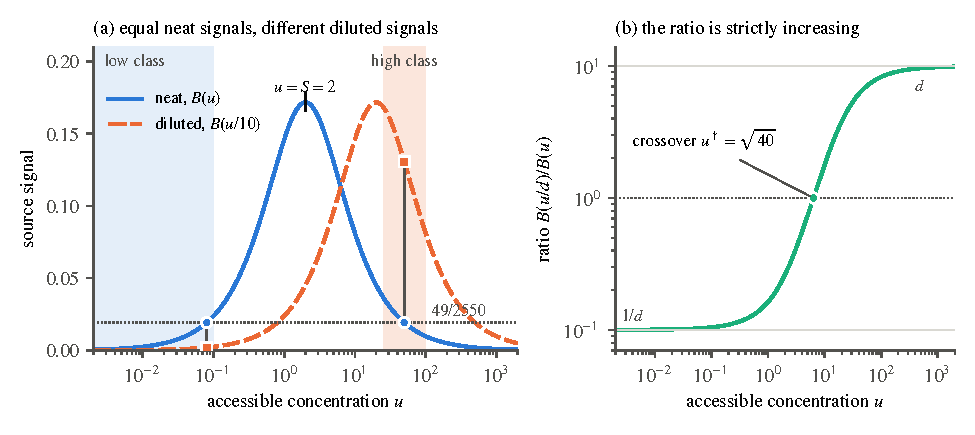
\includegraphics[width=\linewidth]{figures/fig_hook.pdf}
\caption{Synthetic source responses for $C=D=K=J=1$ and $d=10$. (a) The marked
states \eqref{eq:collision} have equal neat signals and different diluted signals;
the neat curve is symmetric under $u\mapsto4/u$. (b) The ratio $B(u/d)/B(u)$
increases strictly from $1/d$ to $d$; with $r=1$ the contrast changes sign at
$u^\dagger=\sqrt{40}$. Floating-point illustration; the statements are proved in
Section~\ref{sec:structure}.}
\label{fig:hook}
\end{figure}

\begin{theorem}[Unimodality, two preimages, monotone ratio; \Conv]\label{thm:structure}
Fix $C,D,K,J>0$ and $d>1$.
\begin{enumerate}[label=(\roman*),leftmargin=2.2em,itemsep=1pt]
\item $E_C=1-Kp/(C(1-p)^2+Kp^2)$; it increases strictly from $0$ to $1$ on
$(0,\infty)$, and $L_B=1-E_C-E_D$ decreases strictly from $1$ to $-1$.
\item $B$ is strictly increasing on $(0,u^*]$ and strictly decreasing on
$[u^*,\infty)$ for a unique $u^*$, with $B(0^+)=B(\infty)=0$. Every level
$s\in(0,B(u^*))$ has exactly two preimages $u_-(s)<u^*<u_+(s)$.
\item The ratio $R(u)=B(u/d)/B(u)$ is strictly increasing, with $R(0^+)=1/d$ and
$R(\infty)=d$.
\item For $1/d<r<d$ there is a unique crossover $u^\dagger$ with $R(u^\dagger)=1/r$,
and $\Delta(u)<0$ for $0<u<u^\dagger$ while $\Delta(u)>0$ for $u>u^\dagger$.
\end{enumerate}
\end{theorem}
\begin{proof}
Differentiating $C=up+Kp/(1-p)$ gives $p'=-p/(u+K/(1-p)^2)<0$, so
$E_C=u(1-p)^2/(u(1-p)^2+K)$. Substituting $u(1-p)^2=(1-p)(C(1-p)-Kp)/p$ from the
balance, and writing $Q=C(1-p)^2+Kp^2$, the numerator becomes $Q-Kp$ and the
denominator $Q$, hence $E_C=1-Kp/Q$. A direct computation gives
\[
 \frac{\mathrm dE_C}{\mathrm dp}=-\frac{K\{C-(C+K)p^2\}}{Q^2}.
\]
At $u=0$ the balance gives $p=C/(C+K)$, and $p$ decreases in $u$, so
$p^2\le(C/(C+K))^2<C/(C+K)$ and the derivative is negative. Since $p$ decreases in
$u$, $E_C$ increases in $u$. At $p=C/(C+K)$ one finds $Q=CK/(C+K)$ and $Kp/Q=1$, so
$E_C(0^+)=0$; as $u\to\infty$, $p\to0$, $Q\to C$ and $E_C\to1$. This proves (i),
because $\log B=\log u+\log p+\log q$.
For (ii), $L_B$ is continuous and strictly decreasing from $1$ to $-1$, so it has a
unique zero $u^*$; the limits of $B$ follow from \eqref{eq:envelopes}.
For (iii), $\mathrm d\log R/\mathrm d\log u=L_B(u/d)-L_B(u)>0$ since $u/d<u$. The
limits follow from $B(u)\sim\alpha u$ and $uB(u)\to CD$, both consequences of
\eqref{eq:envelopes}. Finally $\Delta=B(u)\,(rR(u)-1)$ with $B>0$ gives (iv).
\end{proof}

\begin{proposition}[Hook involution; \Lean{} for the first two sentences]\label{prop:involution}
Let $S=C+K$. If $p$ is the capture occupancy at $u>0$, then the capture occupancy
at $S^2/u$ is $up/S$. Consequently, if $C+K=D+J=S$, then
\begin{equation}\label{eq:involution}
 B(S^2/u)=B(u)\qquad\text{for all }u>0,
\end{equation}
the maximum is at $u^*=S$, the two preimages in
Theorem~\ref{thm:structure}\textup{(ii)} are $u_\pm$ with $u_-u_+=S^2$, and for $r=1$
the crossover is $u^\dagger=S\sqrt d$.
\end{proposition}
\begin{proof}
Put $u'=S^2/u$ and $p'=up/S$. Then $u'p'=Sp$ and
\[
 (C-u'p')(1-p')-Kp'=\frac1S\bigl\{(C-Sp)(S-up)-Kup\bigr\}
 =(C-up)(1-p)-Kp=0 ,
\]
using $S=C+K$ in the expansion. Moreover $0<p'=up/S\le C/S<1$ by
\eqref{eq:pbounds}, so $p'$ is the physical root by Lemma~\ref{lem:source}.
With both sites, $B(u')=u'\,(up/S)(uq/S)=upq$. Symmetry of a strictly unimodal
function about $\log u=\log S$ puts the maximum at $S$ and pairs the preimages.
For $r=1$, $\Delta(u)=0$ means $B(u/d)=B(u)$ with $u/d\ne u$, so
$u/d=S^2/u$.
\end{proof}

For unit parameters $S=2$, the peak value is $B(2)=3-2\sqrt2$, and the rational
pair
\begin{equation}\label{eq:collision}
 (u,p,q)=\Bigl(\frac{200}{2499},\frac{49}{100},\frac{49}{100}\Bigr),\qquad
 \Bigl(\frac{2499}{50},\frac1{51},\frac1{51}\Bigr),
 \qquad \frac{200}{2499}\cdot\frac{2499}{50}=4,
\end{equation}
satisfies \eqref{eq:balance} exactly with the common signal $B=49/2550$
(Figure~\ref{fig:hook}a). Their tenfold-diluted signals are approximately
$0.001993$ and $0.130414$. Theorem~\ref{thm:structure} shows that such a collision
is not a feature of special parameters: \emph{every} neat signal below the peak is
produced by exactly two accessible concentrations, one on each limb, and the
diluted-to-neat ratio separates them because it is injective. The rest of the paper
asks how much of this ideal separation survives interval-valued calibration, gain
drift, error and masking.


\section{A robust two-reading certificate}\label{sec:certificate}

\subsection{Main theorem for the near-unit box}
\begin{theorem}[Source separation and noisy decision; \Lean]\label{thm:main}
Assume \eqref{eq:balance}, \eqref{eq:obs} and the box \eqref{eq:box}. Then
\begin{equation}\label{eq:margin}
 u\in[0,\tfrac25]\implies\Delta(u)\le0,\qquad
 u\in[20,100]\implies\Delta(u)\ge\tfrac1{25}.
\end{equation}
Consequently, for the native classes $x\in[0,\tfrac25]$ (low) and $x\in[25,100]$ (high),
\begin{equation}\label{eq:noisy}
 Z\le2\eps\ \text{ on the low class},\qquad
 Z\ge\gmin/25-2\eps\ \text{ on the high class},
\end{equation}
and the rule ``high if and only if $Z>2\eps$'' separates the two classes whenever
$4\eps<\gmin/25$.
\end{theorem}

The source class is nonempty for every $x\ge0$ (take unit parameters, unit gains,
$d=10$ and the physical roots; this is also compiled). The binary conclusion
requires membership in one of the two declared classes; it says nothing about the
guard band between them or about $x>100$. Sections~\ref{sec:unpromised}
and~\ref{sec:limits} treat both.

\begin{proof}
\emph{Low sign.} For $0\le u\le\frac25$, Lemma~\ref{lem:source} with $K+C,J+D\le a:=\frac{11}5$
and $CD\ge\frac{81}{100}$ gives
\[
 B(u)\ge\frac{(81/100)\,u}{(u+11/5)^2}\ge\frac{81}{676}\,u,\qquad
 rB(u/d)\le\frac{21}{20}\cdot\frac u9=\frac7{60}\,u ,
\]
and $\frac7{60}<\frac{81}{676}$. This includes $u=0$.

\emph{Retaining the shared reagent product.} Let $r_0=\frac{19}{20}$. For $u>0$,
Lemma~\ref{lem:source} applied at $u/d$ and at $u$ gives
$B(u/d)\ge CD\,du/(u+ad)^2$ and $B(u)\le CD/u$ with the \emph{same} factor $CD$, so
\begin{equation}\label{eq:shared}
 \Delta(u)\ge CD\Bigl\{\frac{r_0du}{(u+ad)^2}-\frac1u\Bigr\}.
\end{equation}
For a target margin $m>0$ define
\begin{equation}\label{eq:poly}
 P_m(u,d)=81\,r_0du^2-(81+100mu)(u+ad)^2 .
\end{equation}
If $P_m(u,d)\ge0$, dividing by $u(u+ad)^2$ shows that the braces in
\eqref{eq:shared} are at least $100m/81\ge0$, and $CD\ge81/100$ then gives
$\Delta\ge m$. No separate maximisation of the neat reagent product is used; doing
so loses a factor of more than thirty in the margin (Remark~\ref{rem:tight}).

\emph{Two dilution endpoints suffice.} $P_m$ is a concave quadratic in $d$, and for
$9\le d\le11$ direct expansion gives
\begin{equation}\label{eq:interp}
 P_m(u,d)=\tfrac{11-d}{2}P_m(u,9)+\tfrac{d-9}{2}P_m(u,11)
 +\tfrac{121}{25}(81+100mu)(d-9)(11-d),
\end{equation}
whose last term is nonnegative.

\emph{Eight coefficients.} At either endpoint $P_m$ is a cubic in $u$. With
$u=20+80t$, $0\le t\le1$, and $m=\frac1{25}$,
\begin{equation}\label{eq:bern}
 P_m(u,d)=b_0(1-t)^3+3b_1t(1-t)^2+3b_2t^2(1-t)+b_3t^3
\end{equation}
identically in $t$, with the coefficients of Table~\ref{tab:coefficients}. All are
positive and every Bernstein basis function is nonnegative on $[0,1]$
\cite{farouki2012,garloff1993}, so $P_m\ge0$ on the whole rectangle
$[20,100]\times[9,11]$. These are polynomial identities over the reals, not sampled
corner tests.

\emph{Native classes and noise.} For $\rho\in[\frac45,1]$, $x\le\frac25$ implies
$u\le\frac25$ and $x\in[25,100]$ implies $u\in[20,100]$. Finally
$Z=g\Delta+e_d-e_1$ with $|e_d-e_1|\le2\eps$; $g>0$ preserves the low sign and
$g\ge\gmin$ the high bound.
\end{proof}

\begin{table}[t]
\centering\small
\caption{Exact Bernstein coefficients in \eqref{eq:bern} for the $0.04$ source margin.}
\label{tab:coefficients}
\begin{tabular}{@{}ccccc@{}}\toprule
$d$ & $b_0$ & $b_1$ & $b_2$ & $b_3$\\\midrule
$9$ & $549739/25$ & $6249899/25$ & $23318059/25$ & $554219/25$\\
$11$ & $601099/25$ & $25425377/75$ & $34047819/25$ & $26119179/25$\\\bottomrule
\end{tabular}
\end{table}

\subsection{General calibration boxes}\label{sec:general}
Nothing in the argument depends on the parameters being near one.

\begin{theorem}[General-box certificate; \Lean]\label{thm:general}
Let $C,D,K,J>0$ satisfy $K+C\le A$, $J+D\le H$ and $CD\ge c>0$, let $u>0$, $d>0$,
$r\ge r_0\ge0$ and $m\ge0$, and put
\begin{equation}\label{eq:general}
 Q_m(u,d)=c\,r_0\,d\,u^2-(c+mu)(u+Ad)(u+Hd).
\end{equation}
\begin{enumerate}[label=(\roman*),leftmargin=2.2em,itemsep=1pt]
\item If $Q_m(u,d)\ge0$ then $\Delta(u)=rB(u/d)-B(u)\ge m$.
\item For $d_-\le d\le d_+$,
$(d_+-d_-)\,Q_m(u,d)=(d_+-d)\,Q_m(u,d_-)+(d-d_-)\,Q_m(u,d_+)
+(d_+-d_-)AH(c+mu)(d-d_-)(d_+-d)$; hence nonnegativity at the two dilution
endpoints implies nonnegativity on $[d_-,d_+]$.
\item If $0\le u\le u_L$, $d\ge d_{\min}>0$, $0\le r\le r_{\max}$ and
\begin{equation}\label{eq:lowsign}
 r_{\max}\,(u_L+A)(u_L+H)\le c\,d_{\min},
\end{equation}
then $\Delta(u)\le0$.
\end{enumerate}
\end{theorem}
\begin{proof}
(i) is the argument leading to \eqref{eq:shared} with $(u+Ad)(u+Hd)$ in place of
$(u+ad)^2$: $Q_m\ge0$ is equivalent to
$c\{r_0du/((u+Ad)(u+Hd))-1/u\}\ge m$, and $CD\ge c$. (ii) is an identity for a
quadratic in $d$ with leading coefficient $-AH(c+mu)\le0$. For (iii),
$B(u)\ge cu/((u_L+A)(u_L+H))$ by \eqref{eq:envelopes} and
$rB(u/d)\le r_{\max}u/d_{\min}$ by $B(v)\le v$.
\end{proof}

For a box of calibration intervals one takes $A=K_{\max}+C_{\max}$,
$H=J_{\max}+D_{\max}$, $c=C_{\min}D_{\min}$ and $r_0=r_{\min}$. On a concentration
interval $[L,U]$ the endpoint cubics $Q(u)=Q_m(u,d_\pm)$ have Bernstein coefficients
\begin{equation}\label{eq:bernformula}
 b_0=Q(L),\quad b_1=Q(L)+\tfrac{U-L}3Q'(L),\quad
 b_2=Q(U)-\tfrac{U-L}3Q'(U),\quad b_3=Q(U),
\end{equation}
so a complete design check is the evaluation of eight rational numbers. A negative
coefficient means that this sufficient certificate failed, not that the
observations overlap; a narrower calibration box, a smaller margin or a subdivision
of $[L,U]$ can then be tried. Theorem~\ref{thm:main} is the instance $A=H=\frac{11}5$,
$c=\frac{81}{100}$, for which $P_m=100\,Q_m$.

\paragraph{Operating alternatives for the near-unit box.} Table~\ref{tab:ranges}
lists four compiled certificates. Each row is a separate guarantee: the best
threshold, range and margin of different rows cannot be combined. The low class is
$[0,\frac25]$ throughout.

\begin{table}[t]
\centering\small
\caption{Certified alternatives for the near-unit box \eqref{eq:box}. The error
condition is for equal per-reading allowances and $\gmin=1$; it is an absolute
normalised signal allowance, not a coefficient of variation.}
\label{tab:ranges}
\begin{tabular}{@{}cccc@{}}\toprule
Accessible high range & Native high range & Source margin $m$ & Error condition\\\midrule
$[20,100]$ & $[25,100]$ & $0.04$ & $\eps<0.01$\\
$[12,100]$ & $[15,100]$ & $0.01$ & $\eps<0.0025$\\
$[20,1000]$ & $[25,1000]$ & $0.005$ & $\eps<0.00125$\\
$[20,10000]$ & $[25,10000]$ & $0.0005$ & $\eps<0.000125$\\\bottomrule
\end{tabular}
\end{table}

\begin{proposition}[Uniform range law; \Lean]\label{prop:allU}
For the near-unit box, $u\ge20$, $d\in[9,11]$ and $r\ge\frac{19}{20}$,
\begin{equation}\label{eq:allU}
 u\,\Delta(u)\ge\frac{7371}{8000},\qquad\text{so}\qquad
 \Delta(u)\ge\frac{7371}{8000\,U}\quad\text{on }20\le u\le U .
\end{equation}
\end{proposition}
\begin{proof}
By \eqref{eq:shared}, $u\Delta\ge CD\{r_0\,d/(1+11d/(5u))^2-1\}$. For $u\ge20$ the
denominator is at most $(1+11d/100)^2$, and $4d-9(1+11d/100)^2$ is a concave
quadratic with values $\frac{3591}{10000}$ and $\frac{431}{10000}$ at $d=9,11$; hence
$d/(1+11d/(5u))^2\ge\frac94$ and
$u\Delta\ge\frac{81}{100}(\frac{19}{20}\cdot\frac94-1)=\frac{7371}{8000}$.
\end{proof}

Figure~\ref{fig:ceiling} compares the finite-range certificates with
\eqref{eq:allU}. Neither is an optimal frontier.

\begin{figure}[t]
\centering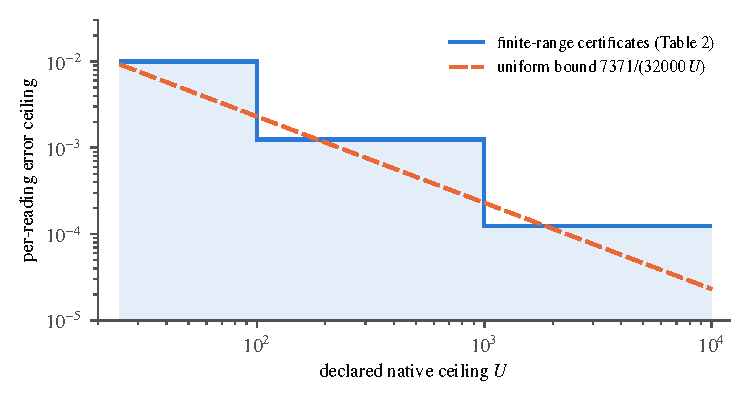
\includegraphics[width=.72\linewidth]{figures/fig_ceiling.pdf}
\caption{Sufficient per-reading error ceilings for the native high range $[25,U]$,
$\rho\in[0.8,1]$ and $\gmin=1$. Steps: Table~\ref{tab:ranges}. Dashed: the uniform
law \eqref{eq:allU}, i.e.\ $\eps<7371/(32000\,U)$. Strictly smaller errors are
certified.}
\label{fig:ceiling}
\end{figure}

\subsection{Capacities a hundred times the dissociation constants}
Immunoassay reagents are often used at capacities far above their dissociation
constants. The following synthetic design regimes show that the certificate is not
confined to comparable scales. They are not measured parameters of any commercial
assay.

\begin{example}[High capacity; \Lean]\label{ex:A}
Take $c_0=1$~nM and
\[
 C,D\in[9,11]\ \text{nM},\qquad K,J\in[0.09,0.11]\ \text{nM},
\]
with $d\in[9,11]$, $r\in[\frac{19}{20},\frac{21}{20}]$, $\rho\in[\frac45,1]$. The
capacity-to-affinity ratio lies between about $82$ and $122$. Here
$A=H=\frac{1111}{100}$ and $c=81$. Condition \eqref{eq:lowsign} holds with $u_L=15$
since $\frac{21}{20}(26.11)^2\approx715.8\le729$, and the eight Bernstein
coefficients of $Q_{2/5}$ on $[100,1000]$ are positive (Appendix~\ref{app:coeff}).
Therefore
\begin{equation}\label{eq:exA}
 x\le15\ \text{nM}\implies\Delta\le0,\qquad
 125\ \text{nM}\le x\le1000\ \text{nM}\implies\Delta\ge\tfrac25 ,
\end{equation}
and with $\gmin=1$ the decision survives any equal per-reading error $\eps<0.1$ in
the normalised signal scale (one signal unit is the reading of $1$~nM of doubly
bound analyte at unit gain). A second certificate for the same box gives margin
$\frac3{20}$ on accessible $[60,1000]$, that is, native high class $[75,1000]$~nM for
$\eps<0.0375$. Table~\ref{tab:exA} gives central illustrations. The high class
deliberately exceeds the reagent capacity: reagent excess over a normal measuring
range is not reagent excess over every out-of-range specimen.
\end{example}

\begin{table}[t]
\centering\small
\caption{Example~\ref{ex:A} at the central parameters $C=D=10$, $K=J=0.1$~nM,
$\rho=0.8$, $d=10$, unit gains. Floating-point illustration; the proof is the
coefficient table in Appendix~\ref{app:coeff}.}
\label{tab:exA}
\begin{tabular}{@{}rrrrr@{}}\toprule
Native $x$ (nM) & Accessible $u$ (nM) & Neat $B(u)$ & Diluted $B(u/10)$ & Contrast\\\midrule
$1$ & $0.8$ & $0.782904$ & $0.078411$ & $-0.704493$\\
$125$ & $100$ & $0.997782$ & $8.187989$ & $7.190207$\\
$500$ & $400$ & $0.249872$ & $2.483435$ & $2.233563$\\
$1000$ & $800$ & $0.124968$ & $1.246437$ & $1.121469$\\\bottomrule
\end{tabular}
\end{table}

\begin{example}[Unequal capacities; \Lean]\label{ex:B}
Let $C\in[9,11]$, $D\in[18,22]$, $K\in[0.09,0.11]$, $J\in[0.18,0.22]$~nM, so that
$A=\frac{1111}{100}$, $H=\frac{1111}{50}$, $c=162$. Then \eqref{eq:lowsign} holds with
$u_L=20$ ($\frac{21}{20}\cdot31.11\cdot42.22\approx1379\le1458$) and $Q_{4/5}$ has
positive Bernstein coefficients on $[200,1000]$: native $x\le20$~nM gives
$\Delta\le0$, native $x\in[250,1000]$~nM gives $\Delta\ge\frac45$, and $\eps<0.2$
suffices at $\gmin=1$. The classes and signal scales differ from those of
Example~\ref{ex:A}, so the margins $0.8$, $0.4$ and $0.04$ are not a ranking of designs.
\end{example}

\begin{figure}[t]
\centering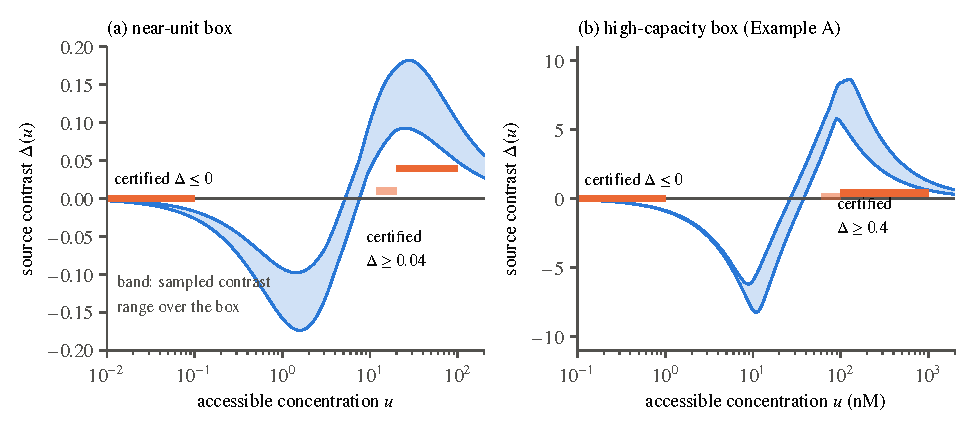
\includegraphics[width=\linewidth]{figures/fig_margins.pdf}
\caption{Certified statements (thick segments) against the range of the source
contrast sampled over the corners of the calibration box (band). (a)
Near-unit box: $\Delta\le0$ on $[0,0.4]$ (shown from $0.01$), $\Delta\ge0.04$ on
$[20,100]$, and the alternative $\Delta\ge0.01$ from $12$ (faint). (b)
Example~\ref{ex:A}: $\Delta\le0$ up to $15$~nM (shown to $1$), $\Delta\ge0.4$ on
$[100,1000]$~nM and $\Delta\ge0.15$ from $60$~nM (faint). The band is a numerical
illustration.}
\label{fig:margins}
\end{figure}

\begin{remark}[Tightness and the necessary guard band; numerical]\label{rem:tight}
The admissible state $u=100$, $d=9$, $C=D=\frac9{10}$, $K=J=\frac{11}{10}$,
$r=\frac{19}{20}$ has $\Delta\approx0.0486095$, and a multistart search finds no
smaller value on the high class, so the certified $0.04$ is about $82\%$ of the
best possible uniform margin. The corresponding figures for Examples~\ref{ex:A}
and~\ref{ex:B} are $0.4$ against about $0.610$ and $0.8$ against about $1.218$. An earlier version of the argument, which bounded the two readings
independently, certified only $\frac3{2500}$; retaining the shared product $CD$
improved the guarantee by a factor of $100/3$ without changing any assumption. By
Theorem~\ref{thm:structure}(iv) the sign of $\Delta$ flips at the crossover
$u^\dagger$, which depends on the unknown parameters: over the corners of the
near-unit box it ranges numerically over about $[5.20,7.58]$, and over
$[26.6,37.8]$~nM for Example~\ref{ex:A}. No sign-based rule can therefore have an
accessible low threshold above, or a high threshold below, those intervals; a
guard band is intrinsic, not an artefact of the proof.
\end{remark}

\section{From source margins to decisions}\label{sec:decisions}

\subsection{Error budgets}
\begin{proposition}[Noise wrapper; \Lean{} for equal allowances]\label{prop:noise}
Suppose a source statement gives $\Delta\le0$ on a low class and $\Delta\ge m$ on a
high class, and $|e_1|\le\eps_1$, $|e_d|\le\eps_d$, $g\ge\gmin>0$. Then
$Z\le\eps_1+\eps_d$ on the low class and $Z\ge\gmin m-\eps_1-\eps_d$ on the high
class; the threshold rule is correct whenever $2(\eps_1+\eps_d)<\gmin m$. If instead
a direct bound $|e_d-e_1|\le\delta$ is available, $\gmin m>2\delta$ suffices.
\end{proposition}
A truly shared additive offset cancels in $Z$ and must not be counted twice;
different specimen backgrounds must not be assumed to cancel.

\subsection{Reporting without a binary promise}\label{sec:unpromised}
For the concrete contract $\gmin=1$, $\eps=10^{-4}$ put $a_*=\frac1{5000}$ and
$b_*=\frac{199}{5000}$.

\begin{corollary}[One-sided exclusions; \Lean]\label{cor:unpromised}
Under the near-unit contract, with no assumption on the class of $x$,
\begin{equation}\label{eq:exclude}
 Z>a_*\implies x>\tfrac1{10},\qquad Z<b_*\implies x\notin[25,100].
\end{equation}
If a ceiling $x\le100$ is independently justified, $a_*<Z<b_*$ implies
$\frac1{10}<x<25$.
\end{corollary}
The inequalities are strict contrapositives of \eqref{eq:noisy}. Neither
$Z\le a_*$ nor $Z\ge b_*$ alone establishes the corresponding class. (The compiled
statement uses the low threshold $\frac1{10}$; by \eqref{eq:margin} the same holds with
$\frac25$.)

\paragraph{Outer enclosures.} Let $\compatible(y_1,y_d)$ be the set of native
concentrations for which some admissible parameters, gains and errors reproduce the
readings, and $\compatible_U=\compatible\cap[0,U]$ for a declared ceiling $U$. The
true concentration always belongs to $\compatible$, and to $\compatible_U$ if
$x\le U$ (\Lean). An implementation that computes an outer set
$\outerset_U\supseteq\compatible_U$ may therefore report, in this order:
\emph{incompatible} if $\outerset_U=\emptyset$; \emph{low} if
$\outerset_U\subseteq[0,0.1]$; \emph{high} if $\outerset_U\subseteq[25,U]$; and
\emph{unresolved} otherwise. Our exact-rational implementation bisects accessible
concentration, in the manner of interval branch-and-prune \cite{moore2009}. For a
cell $[l,h]$ it evaluates the necessary conditions obtained from
\eqref{eq:envelopes} on the cell, from $d\in[9,11]$ and $r\in[\frac{19}{20},\frac{21}{20}]$,
and from the two observation intervals; each reading constrains the \emph{same}
gain $g\ge1$, and the two gain intervals are intersected before a cell is retained.
The contrast cuts \eqref{eq:exclude} are further necessary tests. A cell is
discarded only if a necessary condition fails on all of it, the two halves cover
their parent, and a surviving cell $[l,h]$ projects to the native set
$[l,\frac54h]\cap[0,U]$. By induction on depth every admitted true state survives:
finite depth affects tightness, never soundness (\Conv). A retained cell is not
asserted to be feasible, and the program is not itself formally verified. It keeps
disconnected sets, accepts missing or censored readings as intervals, and abstains
when no finite ceiling is supplied rather than replacing infinity by a large number.

\subsection{From a precision profile to an error allowance}\label{sec:precision}
Assay imprecision is usually reported as a coefficient of variation along the
measuring range \cite{dudley1985,sadler1988}. A coefficient of variation is a
standard-deviation statement, a deterministic bound $|e|\le\eps$ is not, and a
normal error has no finite bound that holds with probability one \cite{gum2008}.
The bridge has two layers. The decision is correct whenever all calibration and
error assumptions hold; a separate measurement model states how often they hold.

Write $e_j=\beta_j'+\xi_j$ with a justified residual-bias bound
$|\beta_j'|\le\beta_j$ and, at the relevant state, $\xi_j$ centred normal with
standard deviation at most $\sigma_j$. With
\begin{equation}\label{eq:coverage}
 k=\Phi^{-1}(1-\alpha/4),\qquad\eps_j=\beta_j+k\sigma_j\quad(j=1,d),
\end{equation}
each of the four tail events has probability at most $\alpha/4$, and the union
bound gives simultaneous coverage at least $1-\alpha$ without any independence
assumption. The resulting guarantee is a repeated-experiment coverage for each fixed
specimen state. It is not a posterior probability of ``low'' or ``high'', and not an
error rate conditional on having selected specimens with unusually low first
readings. Estimated standard deviations need their own confidence or tolerance
construction, and unknown calibration quantities consume their own share of
$\alpha$.

\begin{example}[Synthetic budget]\label{ex:cv}
For the $m=0.04$ certificate suppose that both true normalised means are at most
$0.2$, that the random standard deviation is at most $1\%$ of signal (hence at most
$0.002$, blank noise included) and that each residual bias is at most $0.001$. For
$\alpha=0.01$, $k\approx2.807034$ and $\eps\approx0.00661407<0.01$: the decision is
correct on an event of probability at least $99\%$, with admissible contrast bounds
about $0.01323$ (low) and $0.02677$ (high). If the contrast is calibrated directly,
independent errors give the two-sided $99\%$ allowance
$\delta=0.002+\Phi^{-1}(0.995)\sqrt2\,(0.002)\approx0.00928555<m/2$; in general
$\operatorname{Var}(\xi_d-\xi_1)=\sigma_d^2+\sigma_1^2-2\operatorname{Cov}(\xi_d,\xi_1)$
and the covariance term may not be dropped \cite{gum2008}.
\end{example}
Near the blank a coefficient of variation is unstable and an absolute component is
needed, e.g.\ $\sigma(s)^2=\sigma_0^2+(vs)^2$. Replicates reduce only the independent
random component.

\subsection{Bounded relative error is gain drift}
An unbounded common gain makes a global absolute standard deviation unnatural.
Suppose instead
\begin{equation}\label{eq:relobs}
 Y_1=gB(u)(1+\xi_1)+a_1,\qquad Y_d=grB(u/d)(1+\xi_d)+a_d,
 \qquad|\xi_1|,|\xi_d|\le\eta<1,\quad|a_1|,|a_d|\le\eps_0 .
\end{equation}
\begin{proposition}[Relative-error reduction; \Lean]\label{prop:relative}
With $g'=g(1+\xi_1)$ and $r'=r(1+\xi_d)/(1+\xi_1)$ the readings \eqref{eq:relobs}
have exactly the form \eqref{eq:obs}, with
\begin{equation}\label{eq:relbounds}
 g'\ge\gmin(1-\eta),\qquad
 r'\in\Bigl[r_{\min}\frac{1-\eta}{1+\eta},\ r_{\max}\frac{1+\eta}{1-\eta}\Bigr].
\end{equation}
For the near-unit box and $\eta=\frac3{100}$ this interval is
$[\frac{1843}{2060},\frac{2163}{1940}]$; the low sign persists on $[0,\frac1{10}]$
because $\frac{2163}{1940}\cdot\frac19=\frac{721}{5820}<\frac3{20}$, the source margin
on $[20,100]$ is at least $\frac3{100}$, and
\[
 Z\le2\eps_0\ \text{ (low)},\qquad
 Z\ge\tfrac{97}{100}\cdot\tfrac3{100}\,\gmin-2\eps_0\ \text{ (high)}.
\]
\end{proposition}
Relative imprecision thus consumes the gain-drift budget, and the certificate must
be recomputed on the wider interval; the old margin must not be kept. At $\gmin=1$
and $\eps_0=0.001$ the bounds are $0.002$ and $0.0271$. A $3\%$ relative
\emph{envelope} is not a $3\%$ coefficient of variation: for centred normal
relative errors with standard deviation $1\%$ the envelope holds for both readings
with probability at least $1-4\Phi(-3)\approx0.9946$. The same fluctuation must not
be counted in both $r$ and $\xi$.

\section{Exact limits on inference}\label{sec:limits}
Each obstruction below is an observational equivalence: two admissible worlds
produce identical data. They point to different remedies, and only one of them is
cured by more precise measurement.

\subsection{A neat reading alone}
\begin{proposition}[Neat collision; \Lean]\label{prop:neat}
The states \eqref{eq:collision} satisfy \eqref{eq:balance} for unit parameters,
have equal signals, and with $\rho=1$ lie in the low and high classes of
Theorem~\ref{thm:main}. With equal gains and zero error no function of the neat
reading classifies both correctly.
\end{proposition}
By Theorem~\ref{thm:structure}(ii) the same happens for every parameter choice and
every pair $u_\pm(s)$ that straddles the declared classes, and no amount of
replication of the neat reading helps. The statement concerns nonabstaining rules
that must start from this neat reading. It does not rule out a redesigned single
reading, and it is fully consistent with upfront-dilution workflows \cite{wu2018}.
Calibrators, blanks, specimen volume and incubation time are separate costs.

\subsection{Accessible spikes do not identify native availability}
Suppose a post-dilution spike $s$ is fully accessible while native masking
persists, so that every permitted response is a function of $\rho x/d+s$.

\begin{proposition}[Masking; \Lean]\label{prop:mask}
The worlds $(x,\rho)=(\frac1{10},1)$ and $(100,\frac1{1000})$ induce the same response
for every dilution $d$, every spike $s$ and every response function. Hence no
rule on the complete action--response map, and in particular no deterministic
adaptive choice of spikes and dilutions, separates them. More generally, if
$0<\rho_{\min}\le\rho\le\rho_{\max}$ and $\rho_{\min}H\le\rho_{\max}L$, the native
states $(H,\rho_{\min})$ and $(\rho_{\min}H/\rho_{\max},\rho_{\max})$ have the same
accessible concentration, the second lies in the class $x\le L$, and an accessible
interval $[u_-,u_+]$ yields exactly
\begin{equation}\label{eq:projection}
 x\in[u_-/\rho_{\max},\ u_+/\rho_{\min}] .
\end{equation}
\end{proposition}
Spike recovery can be ideal on the accessible scale in both worlds; the second
world lies outside the availability contract of Theorem~\ref{thm:main}, as it must.
For $L>0$, a necessary condition for separating $x\le L$ from $x\ge H$ from
accessible-only measurements is $H/L>\rho_{\max}/\rho_{\min}$, and for exactly known
$u$ both endpoints of \eqref{eq:projection} are attained. Under $\rho\in[0.8,1]$ the
residual factor is $1.25$; once it dominates, a native-recovery measurement is
worth more than a more precise repeat of the same accessible signal. This is a
statement about the stated action model. A spike that demonstrably behaves like
native analyte under a quantified preparation (the premise of parallelism and
recovery validation \cite{desilva2003,ichm10}) supplies different information and
must be modelled as such.

\subsection{A finite panel cannot exclude an unbounded noisy tail}
\begin{proposition}[Blank-compatible tail; \Lean]\label{prop:tail}
For the near-unit reagent box, unit gain, $\rho=1$ and any dilution $0<d\le M$,
\begin{equation}\label{eq:tail}
 0\le B(x/d)\le\frac{121\,d}{100\,x}\le\frac{121M}{100x},
\end{equation}
so if $\eps>0$ and $x\ge121M/(100\eps)$ the all-zero transcript lies within the
error allowance of every reading of the panel, exactly as it does for a blank.
\end{proposition}
The same argument applies along the finite all-blank path of a deterministic
adaptive procedure. No claim is made for randomised protocols, unbounded dilution
ranges or additional measurement channels. For $M=11$ and $\eps=10^{-4}$ every
$x\ge133100$ is blank-compatible (Figure~\ref{fig:blank}). Combined with
Proposition~\ref{prop:allU}: at a fixed bounded dilution range and error model, the
ceilings that can be certified and the ceilings that cannot both scale as $1/\eps$.
The constants do not match and no minimax claim is made.

\begin{figure}[t]
\centering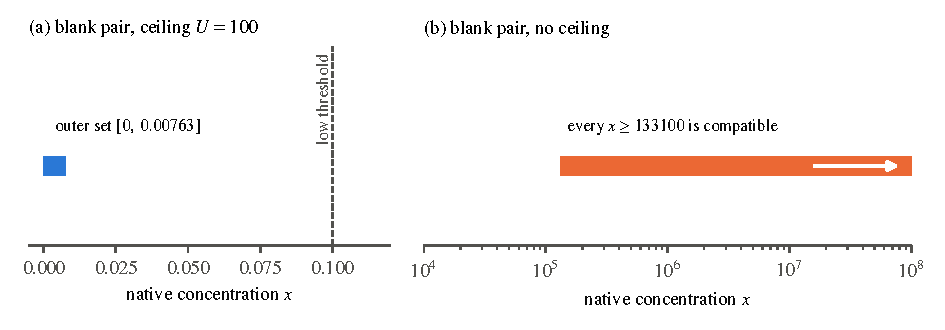
\includegraphics[width=.95\linewidth]{figures/fig_blank.pdf}
\caption{The same pair of blank readings under two domain assumptions ($\gmin=1$,
$\eps=10^{-4}$, dilutions at most $11$). (a) With a declared ceiling $U=100$ the
computed outer set is $[0,125/16384]$, a \emph{low} report. (b) Without a ceiling
every $x\ge133100$ is compatible; the bar shows a subset of the compatible set, which
continues to infinity.}
\label{fig:blank}
\end{figure}

\subsection{Ideal identifiability and the noisy tail are compatible}
By Theorem~\ref{thm:structure}(iii), for known parameters and noise-free readings
the ratio $Y_d/(rY_1)=R(u)$ identifies $u$ exactly, on the whole half-line. There is
no contradiction with Proposition~\ref{prop:tail}: along the tail the ratio
approaches its limit $d$ while both raw signals vanish, and by \eqref{eq:tailexp}
\begin{equation}\label{eq:deltatail}
 \Delta(u)=\frac{CD(rd-1)}{u}-\frac{CD(K+J)(rd^2-1)}{u^2}+O(u^{-3}).
\end{equation}
The sign of the contrast stays positive while its size tends to zero. Injectivity
at every finite state does not give stable identification uniformly over an
unbounded range, and a more powerful fitting algorithm cannot substitute for a
justified concentration ceiling.

\section{Departures from the ideal protocol}\label{sec:physical}

\subsection{Availability that changes on dilution}
Let $u=\rho_1x$ and $\kappa=\rho_d/\rho_1>0$. The diluted accessible concentration
is $\kappa u/d=u/d_{\rm eff}$ with $d_{\rm eff}=d/\kappa$, and for positive interval
bounds $d_{\rm eff}\in[d_-/\kappa_+,\ d_+/\kappa_-]$.

\begin{proposition}[Availability drift; \Lean]\label{prop:drift}
For the near-unit box with $\kappa\in[\frac{19}{20},\frac{21}{20}]$ the effective dilution
lies in $[\frac{60}7,\frac{220}{19}]$, the source margin on $u\in[20,100]$ is at least
$\frac3{100}$, and the low sign persists because $\frac{21}{20}\cdot\frac7{60}<\frac3{20}$.
\end{proposition}
The extension consumes margin, because the dilution interval has really widened.
Shared $C,D,K,J$ and the observation model remain necessary; altered affinities,
nonspecific adsorption and unknown backgrounds are not absorbed by $d_{\rm eff}$.

\subsection{A calibrated attenuation bound suffices}
\begin{proposition}[Transient signals; \Lean]\label{prop:transient}
Suppose the actual source signals satisfy
\begin{equation}\label{eq:attenuation}
 \tfrac9{10}B(u)\le T_1\le B(u),\qquad\tfrac9{10}B(u/d)\le T_d\le B(u/d).
\end{equation}
For the near-unit box, $rT_d-T_1\le0$ for $u\le\frac1{10}$ and
$rT_d-T_1\ge\frac3{100}$ for $u\in[20,100]$; with noise, the high contrast is at least
$\frac3{100}\gmin-2\eps$.
\end{proposition}
For low $u$ the proof uses $[(21/20)/9-(9/10)(3/20)]u\le0$; for high $u$,
$rT_d-T_1\ge(\frac9{10}r)B(u/d)-B(u)$ and the polynomial certificate with
$r_0=\frac{171}{200}$. The multiplicative form matters: $g$ has no upper bound, so a
small source discrepancy is not a small additive signal error.

\subsection{From rate constants to a sufficient incubation time}
Proposition~\ref{prop:transient} leaves open how \eqref{eq:attenuation} is to be
established. Equilibrium calibration alone cannot do it, since scaling all on- and
off-rates by a small factor preserves $K,J$ and slows the dynamics arbitrarily. For
a well-mixed solution-phase reaction, rate constants do suffice.

Consider mass-action kinetics of the four analyte species $A_{ij}$
($i,j\in\{0,1\}$ the occupancies of the capture and detector sites), in which
capture reagent binds either species with a free capture site at rate
$k^C_{\rm on}$ and dissociates at rate $k^C_{\rm off}=Kk^C_{\rm on}$, the detector
likewise with $k^D_{\rm on}$ and $k^D_{\rm off}=Jk^D_{\rm on}$, independently of the
other site. All analyte is unbound at $t=0$. Let $T(t)=A_{11}(t)$ and
\begin{equation}\label{eq:lambda}
 \lambda_C(u)=k^C_{\rm on}\sqrt{\smash[b]{(u-C)^2+2K(u+C)+K^2}},
\end{equation}
with $\lambda_D$ defined analogously.

\begin{theorem}[Kinetic bridge; \Conv]\label{thm:kinetic}
In the setting just described, for every $u>0$:
\begin{enumerate}[label=(\roman*),leftmargin=2.2em,itemsep=1pt]
\item $A_{11}=upq$, $A_{10}=up(1-q)$, $A_{01}=u(1-p)q$, $A_{00}=u(1-p)(1-q)$, where
$p(0)=q(0)=0$ and
\[
 \dot p=k^C_{\rm on}\{(C-up)(1-p)-Kp\},\qquad
 \dot q=k^D_{\rm on}\{(D-uq)(1-q)-Jq\}.
\]
\item $p$ increases to the equilibrium root $p_*$ with
$0\le p_*-p(t)\le p_*e^{-\lambda_C(u)t}$, and similarly for $q$.
\item For all $t\ge0$,
\begin{equation}\label{eq:kinbound}
 \bigl(1-e^{-\lambda_C(u)t}\bigr)\bigl(1-e^{-\lambda_D(u)t}\bigr)\,B(u)\le T(t)\le B(u).
\end{equation}
\item $\lambda_C(u)\ge k^C_{\rm on}\max\{K,\,2\sqrt{CK}\}$ for every $u\ge0$.
\end{enumerate}
\end{theorem}
\begin{proof}
(i) With the product ansatz the free capture reagent is $C-A_{10}-A_{11}=C-up$ and
the free detector is $D-uq$. Substituting, for instance,
\[
 \dot A_{11}=k^C_{\rm on}(C-up)A_{01}-k^C_{\rm off}A_{11}
 +k^D_{\rm on}(D-uq)A_{10}-k^D_{\rm off}A_{11}=u(\dot p\,q+p\,\dot q),
\]
and the other three equations are verified in the same way. The right-hand sides are
polynomial, so the solution of the initial-value problem is unique and equals the
product form.
(ii) Let $f(p)=k^C_{\rm on}\{(C-up)(1-p)-Kp\}$. Then $f(p_*)=0$, $f>0$ on
$[0,p_*)$, and by uniqueness $p(t)<p_*$ for all $t$, so $p$ is increasing. On
$[0,p_*]$,
\[
 f'(p)=-k^C_{\rm on}(u+C+K-2up)\le-k^C_{\rm on}(u+C+K-2up_*)=-\lambda_C(u),
\]
because $up_*$ is the smaller root of $w^2-(u+C+K)w+uC=0$, that is
$2up_*=u+C+K-\sqrt{(u+C+K)^2-4uC}$. By the mean value theorem
$y=p_*-p$ satisfies $\dot y=-f(p)\le-\lambda_Cy$, hence $y\le p_*e^{-\lambda_Ct}$.
(iii) follows from (i), (ii) and $B=up_*q_*$.
(iv) The radicand equals $(u+K-C)^2+4CK\ge4CK$, and also
$(u-C)^2+2K(u+C)+K^2\ge(|u-C|+K)^2\ge K^2$.
\end{proof}

\begin{corollary}[Sufficient incubation; \Conv]\label{cor:incubation}
Let $\lambda_*=\min\{k^C_{\rm on}\max(K,2\sqrt{CK}),\,k^D_{\rm on}\max(J,2\sqrt{DJ})\}$,
minimised over the calibration box. If both reactions are read at a common time
$t\ge3/\lambda_*$, then \eqref{eq:attenuation} holds for every $u\ge0$ and every
$d$, because $(1-e^{-3})^2\approx0.9029$ (the exact requirement is
$\lambda_*t\ge-\log(1-\sqrt{0.9})\approx2.9697$). Proposition~\ref{prop:transient}
then applies.
\end{corollary}
For the near-unit box and for Example~\ref{ex:A} alike, $2\sqrt{CK}\ge1.8$~nM; with
$c_0=1$~nM and $k_{\rm on}=10^6\,{\rm M^{-1}s^{-1}}=10^{-3}\,{\rm nM^{-1}s^{-1}}$ for
both sites this gives $\lambda_*\ge1.8\times10^{-3}\,{\rm s^{-1}}$ and a sufficient
incubation of about $28$ minutes (a synthetic illustration). For unit parameters the bound is
attained as $u\to0$; it is conservative at high concentration, where binding is
fast (Figure~\ref{fig:kinetic}). The theorem is about homogeneous
mass-action kinetics; diffusion-limited surface binding and lateral flow
\cite{qian2003,rey2017} need their own bridge, and a flat measured time trace does
not by itself establish the factorisation in (i).

\begin{figure}[t]
\centering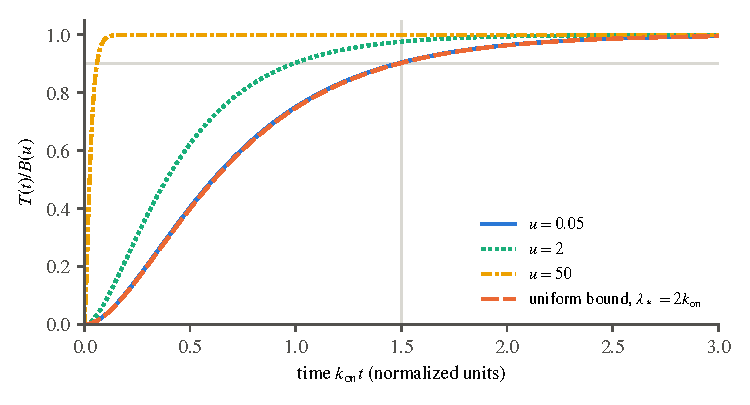
\includegraphics[width=.72\linewidth]{figures/fig_kinetic.pdf}
\caption{Approach to equilibrium of the sandwich concentration for unit parameters
and equal on-rates, against the uniform bound \eqref{eq:kinbound} with
$\lambda_*=2k_{\rm on}$. The $90\%$ level is reached by
$k_{\rm on}t=1.5$ for every concentration. Numerical illustration of
Theorem~\ref{thm:kinetic}.}
\label{fig:kinetic}
\end{figure}

\section{Sequential assays: what washing changes}\label{sec:sequential}
In a sequential (two-step) format the specimen is first incubated with the capture
reagent, unbound material is washed away, and detector is added afterwards
\cite{fernando1992b,wild2013}. Incomplete washing has long been examined as one
source of hook-like behaviour in two-site assays \cite{rodbard1978b,ryall1982}, and
two-step hooks have also been attributed to multiple-epitope interactions that an
antigen-excess partition model does not contain \cite{fernando1992b}. We give an
explicit source model and prove what it implies; it does not describe every
solid-phase assay.

\paragraph{Ideal capture, complete wash.} The captured amount is $w(u)=up(u;C,K)$,
the capture balance of \eqref{eq:balance}, equivalently $Kw=(C-w)(u-w)$. Assume
complete removal of free analyte, perfect retention of captured analyte, a known
detection volume and no loss of capture complexes. Fresh detector with capacity $D$
and constant $J$ then binds the captured analyte with occupancy $q(w;D,J)$, and
\begin{equation}\label{eq:seq}
 \Bseq(u)=w(u)\,q\bigl(w(u);D,J\bigr).
\end{equation}

\begin{theorem}[Ideal washing; \Lean]\label{thm:seq}
$w$ is strictly increasing with $w(u)<\min\{C,u\}$ for $u>0$ and
$0\le w(u_2)-w(u_1)\le u_2-u_1$ for $u_1\le u_2$. Consequently $\Bseq$ is strictly
increasing, and with $b_\infty=C\,q(C;D,J)$,
\begin{equation}\label{eq:plateau}
 0<b_\infty-\Bseq(u)\le\frac{KC}{u-C}\qquad(u>C).
\end{equation}
\end{theorem}
\begin{proof}
If $u_1<u_2$ but $w_1\ge w_2$, then
$Kw_1=(C-w_1)(u_1-w_1)\le(C-w_2)(u_1-w_1)<(C-w_2)(u_2-w_2)=Kw_2$, a contradiction.
If $w_2-w_1>u_2-u_1$, the free analyte decreases while $w$ increases, and
$Kw_2=(C-w_2)(u_2-w_2)<(C-w_1)(u_1-w_1)=Kw_1$ contradicts $w_2>w_1$. The same two
facts for the detector stage show that $b(w)=wq(w;D,J)$ is strictly increasing and
$1$-Lipschitz, so $\Bseq=b\circ w$ is strictly increasing and
$b_\infty-\Bseq(u)\le C-w(u)=Kw/(u-w)\le KC/(u-C)$.
\end{proof}
The ideal response saturates instead of returning to zero: complete washing removes
the free analyte that would compete with captured analyte for detector. Saturation
still destroys quantitative resolution at high $u$, and native masking is unaffected.

\paragraph{Carry-over restores the tail.} Suppose a fraction $\lambda\ge0$ of the
free analyte is carried into the detection stage, $a(u)=\lambda\{u-w(u)\}$ in the
detection-volume convention, and detector binds captured and carried-over
accessible analyte alike. Only detector on captured analyte is read:
\begin{equation}\label{eq:carry}
 B_\lambda(u)=w(u)\,q\bigl(w(u)+a(u);D,J\bigr).
\end{equation}

\begin{proposition}[Carry-over; \Lean]\label{prop:carry}
Let $q_0=q(w;D,J)$ and $q_a=q(w+a;D,J)$ with $a\ge0$. Then $q_a\le q_0$ and
\begin{equation}\label{eq:retention}
 \frac{B_a}{B_0}=\frac{q_a}{q_0}\ge\frac{D}{D+aq_0}\ge\frac{D}{D+a}.
\end{equation}
If $0<\beta\le1$ and $a\beta\le D(1-\beta)$ then $B_a\ge\beta B_0$; in particular
\begin{equation}\label{eq:washspec}
 \lambda_{\max}U\le D_{\min}(\beta^{-1}-1)
 \implies B_\lambda(u)\ge\beta\,\Bseq(u)\quad\text{for }u\le U,\ \lambda\le\lambda_{\max}.
\end{equation}
On the other hand, for every $\lambda>0$ and $u>C$,
\begin{equation}\label{eq:carrytail}
 B_\lambda(u)\le\frac{CD}{\lambda\,(u-C)} .
\end{equation}
\end{proposition}
\begin{proof}
Dividing the detector balance by the occupancy gives $D/q=v+J/(1-q)$ at analyte
level $v$. Occupancy decreases in $v$, so $q_a\le q_0$ and
$D/q_a=w+a+J/(1-q_a)\le D/q_0+a$, which is \eqref{eq:retention}. For the tail,
$(w+a)q_a\le D$, $w\le C$ and $a\ge\lambda(u-C)$ give
$B_\lambda=wq_a\le CD/(w+a)\le CD/(\lambda(u-C))$.
\end{proof}
Thus the limits do not commute: $\lim_{u\to\infty}B_\lambda(u)=0$ for every fixed
$\lambda>0$, whereas $\lim_{\lambda\to0}B_\lambda(u)=\Bseq(u)\to b_\infty>0$. A small
carry-over reintroduces the high-dose mechanism at sufficiently high concentration,
and \eqref{eq:washspec} states how small it must be on a declared range. For example
$D_{\min}=10$~nM, $U=1000$~nM and $\beta=0.9$ require
$\lambda_{\max}\le\frac1{900}\approx0.111\%$ carry-over. This is a model-based
specification that ignores capture loss and matrix changes, and it guarantees signal
retention relative to the ideal washed model, not monotonicity of the imperfectly
washed response. Table~\ref{tab:seq} and Figure~\ref{fig:seq} illustrate it.

\begin{table}[t]
\centering\small
\caption{Sequential model at $C=D=10$, $K=J=0.1$~nM; $b_\infty\approx9.048751$. The
last row is a mathematical tail illustration, not a plausible concentration.}
\label{tab:seq}
\begin{tabular}{@{}rrr@{}}\toprule
Accessible $u$ (nM) & Ideal wash $\Bseq(u)$ & Carry-over $\lambda=10^{-3}$\\\midrule
$1$ & $0.978182$ & $0.978182$\\
$10$ & $8.487565$ & $8.487335$\\
$100$ & $9.043464$ & $9.004325$\\
$1000$ & $9.048271$ & $8.558490$\\
$10^6$ & $9.048750$ & $0.099001$\\\bottomrule
\end{tabular}
\end{table}

\begin{figure}[t]
\centering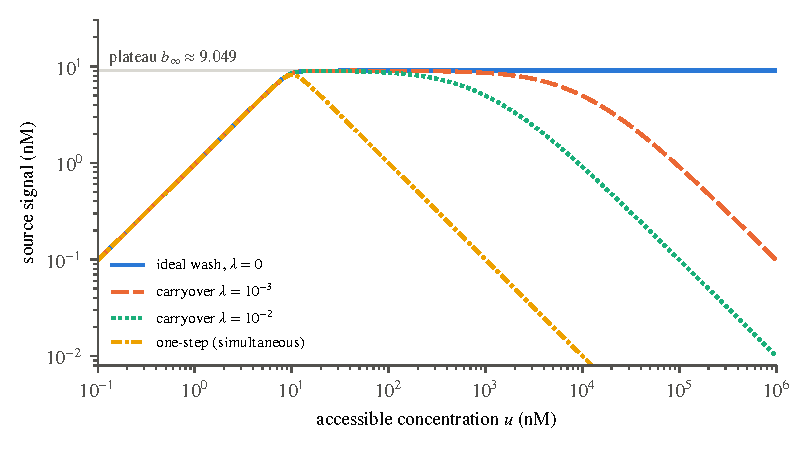
\includegraphics[width=.8\linewidth]{figures/fig_sequential.pdf}
\caption{Synthetic source comparison at $C=D=10$, $K=J=0.1$~nM. Ideal washing gives
a monotone response with plateau $b_\infty$; carry-over fractions $10^{-3}$ and
$10^{-2}$ restore a $1/u$ tail at high concentration; the one-step response
\eqref{eq:balance} hooks as soon as the analyte exceeds the reagent capacity.}
\label{fig:seq}
\end{figure}

\section{Use in assay development}\label{sec:use}
The practical object is a small reproducible calculation, not the inspection of
Bernstein coefficients at the bench.
\begin{enumerate}[leftmargin=2em,itemsep=1pt]
\item \emph{State the decision}: native low and high thresholds, the admitted
ceiling, and whether intermediate concentrations may remain unresolved.
\item \emph{Specify the protocol}: simultaneous or sequential binding, order of
additions, washing, final volumes, read time, raw measured quantity.
\item \emph{Supply external bounds}: site capacities and affinities, availability,
actual dilution, gain drift, linearity, and the error or precision profile; record
which are not independently established. Reagent molecule counts need not equal
binding-site capacities.
\item \emph{Compute a source margin} with Theorem~\ref{thm:general} (eight
coefficients and \eqref{eq:lowsign}), or the sequential source of
Section~\ref{sec:sequential}. If the certificate fails, distinguish a loose bound
from a genuine collision using Theorem~\ref{thm:structure} and Remark~\ref{rem:tight}.
\item \emph{Compare with the observation budget}: simultaneous absolute allowances,
a direct contrast allowance, or the relative-error reduction; allocate probability
only where a stochastic model is supported.
\item \emph{Report the admitted inference}: a promised decision, a one-sided
exclusion, an outer interval, unresolved, or incompatible, together with the domain
and calibration assumptions.
\item \emph{Choose the next informative action}: a matched dilution addresses a
neat collision; native-recovery information addresses masking; a justified ceiling
or an extended validated panel addresses the tail; a wash study addresses carry-over;
an incubation study against Corollary~\ref{cor:incubation} addresses equilibration.
\end{enumerate}

Table~\ref{tab:examples} collects synthetic scenarios. The outer program returns
\emph{high} for unit-source $x=50$ with native enclosure about $[37.415,100]$, and
\emph{incompatible} for a raw reading of $-1$, which violates the nonnegative-source
model by far more than the error allowance; a small negative blank-corrected reading
within $\eps$ is fully compatible. For the low collision state
$x=\frac{200}{2499}$ the outer set is $[0,\frac{1375}{8192}]\approx[0,0.168]$, which is
\emph{unresolved} against the threshold $0.1$ although the promised binary rule
classifies it correctly: an outer enclosure and a promised decision use different
information. A failed control removes the right to use the calibration assumptions
and leads to unresolved reporting, not to a forced label.

\begin{table}[t]
\centering\small
\caption{Worked synthetic scenarios (near-unit box, $\gmin=1$, $\eps=10^{-4}$,
$U=100$ unless stated). Retained intervals are outer relaxations.}
\label{tab:examples}
\begin{tabular}{@{}>{\raggedright\arraybackslash}p{.27\linewidth}>{\raggedright\arraybackslash}p{.33\linewidth}>{\raggedright\arraybackslash}p{.32\linewidth}@{}}\toprule
Observations & Conclusion & Information that matters next\\\midrule
Neat collision \eqref{eq:collision}, matched dilution added & Promised low/high states are separated & None for the binary contract\\
Same neat value, dilution omitted & Two branches remain; unresolved & The matched diluted reading\\
Native $x=1$ & Guard-band state; unresolved & Refine the target or keep the enclosure\\
Two blank readings & With $U=100$: outer set $[0,0.00763]$, low. Without a ceiling: unresolved & Justify a range or change the panel\\
Native masking, ideal accessible spike recovery & Identical data for $x=0.1$ and $x=100$ & Native recovery or changed preparation\\
$\ge90\%$ of equilibrium signal, or $5\%$ availability drift & Source margin $0.03$ & Verify the attenuation (Cor.~\ref{cor:incubation}) or drift bound\\\bottomrule
\end{tabular}
\end{table}

For reflex dilution triggered by a low first reading, ``the contrast rule is sound
once the pair is obtained'' must be kept apart from ``the trigger captures every
relevant high specimen''; the latter needs its own analysis of the first-reading
trigger, its errors and the selection it induces. A study aimed at validating the
model should retain independently prepared specimen identities, raw neat and diluted
signals and backgrounds, actual volumes and timing, run and lot information,
censoring, and an independent native concentration or recovery measurement, and
should deliberately include cases near the weakest calibration assumptions. Repeated
frames of one reaction are not independent specimens. Published dilution studies
\cite{hunsaker2024} report concentrations, not the raw paired signals and binding
calibration that the certificate needs; none of the numbers in this paper is
empirical.

\section{Verification, reproducibility and limitations}\label{sec:verification}
\paragraph{Formal verification.} The \Lean-tagged statements were compiled with
Lean~4 (version 4.30.0) and a pinned mathlib \cite{demoura2021,mathlib2020}.
Compilation treats warnings as errors and accepts neither \texttt{sorry} nor added
axioms; the receipts record source hashes, the toolchain, declaration interfaces
and axiom inventories (the standard \texttt{propext}, \texttt{Classical.choice},
\texttt{Quot.sound} only). Table~\ref{tab:formal} maps statements to declarations in
the namespace \lean{SandwichImmunoassay}. The compiled statements quantify over all
real parameters in the stated intervals and over all physical roots of
\eqref{eq:balance}; no separation margin is assumed, and the finite certificates
prove the stated real rectangles, not a list of samples. What Lean verifies is the
encoded mathematics under its hypotheses. The physical adequacy of
\eqref{eq:balance}, the calibration of any real assay, the Python reporting program
and the correspondence between prose and declarations remain separate
responsibilities; the last was checked by hand against the sources. Formal proof
has been applied to physical chemistry before \cite{bobbin2024}; here its role is
narrow and practical, namely to remove doubt about inequalities that are uniform
over seven real parameters.

\begin{table}[t]
\centering\small
\caption{Statement-to-declaration map (namespace \texttt{SandwichImmunoassay}).}
\label{tab:formal}
\begin{tabular}{@{}>{\raggedright\arraybackslash}p{.33\linewidth}>{\raggedright\arraybackslash}p{.62\linewidth}@{}}\toprule
Statement & Lean module: declarations\\\midrule
Lemma~\ref{lem:source} & \texttt{Source}: \texttt{occupancy\_exists}, \texttt{Occupancy.unique}, \texttt{Occupancy.bounds}, \texttt{Reaction.envelopes}\\
Proposition~\ref{prop:involution}, \eqref{eq:collision} & \texttt{Structure}: \texttt{Occupancy.involution}, \texttt{signal\_involution}; \texttt{Source}: \texttt{source\_endpoint\_collision}\\
Theorem~\ref{thm:main} & \texttt{MarginCertificate}: \texttt{source\_certificate}, \texttt{dilution\_endpoints}, \texttt{noisy\_margin}; \texttt{OperatingRanges}: \texttt{stronger\_margin\_source}; \texttt{GeneralBox}: \texttt{near\_unit\_low\_wide}; \texttt{Publication}: \texttt{publication\_main}; \texttt{Main}: \texttt{specimen\_exists}\\
Theorem~\ref{thm:general} & \texttt{GeneralBox}: \texttt{general\_source\_certificate}, \texttt{general\_dilution\_endpoints}, \texttt{general\_low\_sign}\\
Table~\ref{tab:ranges}, Prop.~\ref{prop:allU} & \texttt{OperatingRanges}: \texttt{smaller\_guard\_source}, \texttt{range\_1000\_source}, \texttt{range\_10000\_source}; \texttt{GeneralBox}: \texttt{uniform\_tail\_margin}\\
Examples~\ref{ex:A}, \ref{ex:B} & \texttt{GeneralBox}: \texttt{capacity\_high}, \texttt{capacity\_guard60}, \texttt{capacity\_low\_wide}, \texttt{capacity\_noisy\_high}, \texttt{capacity\_noisy\_low}, \texttt{unequal\_high}, \texttt{unequal\_low\_wide}\\
Cor.~\ref{cor:unpromised}, truth containment & \texttt{Consequences}: \texttt{excludes\_low}, \texttt{identifies\_guard\_band}, \texttt{truth\_within}; \texttt{Publication}: \texttt{publication\_main}\\
Proposition~\ref{prop:relative} & \texttt{GeneralBox}: \texttt{relative\_error\_reduction}, \texttt{relative\_error\_high}, \texttt{relative\_error\_low}, \texttt{relative\_error\_noisy\_high}, \texttt{relative\_error\_noisy\_low}\\
Props.~\ref{prop:neat}--\ref{prop:tail} & \texttt{Main}: \texttt{endpoint\_no\_classifier}; \texttt{Controls}: \texttt{no\_masking\_classifier}, \texttt{availability\_repair}; \texttt{Preparation}: \texttt{availability\_overlap}; \texttt{Obstructions}: \texttt{tail\_blank}\\
Props.~\ref{prop:drift}, \ref{prop:transient} & \texttt{Preparation}: \texttt{effective\_dilution}, \texttt{transient\_high}, \texttt{transient\_low}, \texttt{transient\_noisy\_high}; \texttt{OperatingRanges}: \texttt{availability\_drift\_source}\\
Theorem~\ref{thm:seq}, Prop.~\ref{prop:carry} & \texttt{Sequential}: \texttt{Occupancy.captured\_strictMono}, \texttt{Occupancy.captured\_lipschitz}, \texttt{sequential\_strictMono}, \texttt{sequential\_below\_plateau}, \texttt{sequential\_plateau\_gap}, \texttt{carryover\_retention}, \texttt{wash\_specification}, \texttt{carryover\_tail}\\
Thms.~\ref{thm:structure}, \ref{thm:kinetic}, Cor.~\ref{cor:incubation}, enclosure soundness & Conventional proofs in this paper\\\bottomrule
\end{tabular}
\end{table}

\paragraph{Reproducibility.} The source package contains the manuscript, the figure
and table generators, the exact-rational enclosure program, and a script that
replays every number printed in this paper: the Bernstein identities and low-sign
conditions in exact arithmetic, and the floating-point illustrations, the
involution, the elasticity formula, the monotone ratio, the kinetic bound (against
an ODE solver, including the four-species system) and the sequential bounds
numerically. The Lean modules and their receipts accompany the repository.
Generated curves are synthetic; no clinical dataset is used.

\paragraph{Limitations.} The certificates are sufficient, not sharp; the constants
in the $1/\eps$ range law do not match the obstruction; and the structure theorem
and the kinetic bridge are not yet formalised. The model is homogeneous,
noncooperative and two-site. Immobilised-site calibration, multivalency and avidity,
cooperative binding \cite{roy2017}, transport and residence time in lateral flow
\cite{qian2003,ross2020}, heterophilic and matrix interference
\cite{selby1999,tate2004,sturgeon2011}, native commutability and clinical
performance all lie outside it. Chemiluminescence is a readout modality and not
evidence for a binding protocol, and a lateral-flow control line is not an invariant
gain standard \cite{ross2020}. The practical use of the results is to state what an
assay must calibrate, what two readings can then exclude, and which missing
information cannot be recovered by repeating an indistinguishable control.

\appendix
\section{Exact certificate coefficients}\label{app:coeff}
Table~\ref{tab:allcoeff} lists the Bernstein coefficients \eqref{eq:bernformula} of
$Q_m(\cdot,d_\pm)$ in the normalisation \eqref{eq:general} for every certificate used
in the paper. Near-unit rows have $A=H=\frac{11}5$, $c=\frac{81}{100}$ (so that
$P_m=100\,Q_m$, the normalisation of Table~\ref{tab:coefficients} and of the Lean
sources) and $r_0=\frac{19}{20}$ unless stated; Example~\ref{ex:A} has
$A=H=\frac{1111}{100}$, $c=81$; Example~\ref{ex:B} has $A=\frac{1111}{100}$,
$H=\frac{1111}{50}$, $c=162$. All coefficients are positive; the smallest, $447/2500$,
occurs for the $[12,100]$ certificate at $d=11$, which indicates how little room
that alternative has.

\begin{table}[ht]
\centering\scriptsize
\renewcommand{\arraystretch}{1.15}\setlength{\tabcolsep}{3pt}
\caption{Bernstein coefficients of all certificates (exact rationals).}
\label{tab:allcoeff}
\resizebox{\linewidth}{!}{\begin{tabular}{@{}llllll@{}}\toprule
certificate & $d$ & $b_0$ & $b_1$ & $b_2$ & $b_3$\\\midrule
$m=\tfrac1{25}$, $[20,100]$ & $9$ & $549739/2500$ & $6249899/2500$ & $23318059/2500$ & $554219/2500$\\
 & $11$ & $601099/2500$ & $25425377/7500$ & $34047819/2500$ & $26119179/2500$\\
\addlinespace[2pt]
$m=\tfrac1{100}$, $[12,100]$ & $9$ & $142047/2500$ & $7251831/2500$ & $9789651/500$ & $108194519/2500$\\
 & $11$ & $447/2500$ & $26997893/7500$ & $2477943/100$ & $141811479/2500$\\
\addlinespace[2pt]
$m=\tfrac1{200}$, $[20,10^3]$ & $9$ & $3321809/2500$ & $163930579/2500$ & $4820411849/2500$ & $2207865619/2500$\\
 & $11$ & $4019969/2500$ & $620561017/7500$ & $6102058209/2500$ & $5924733579/2500$\\
\addlinespace[2pt]
$m=\tfrac1{2000}$, $[20,10^4]$ & $9$ & $1839109/1250$ & $351625757/500$ & $126741925313/625$ & $273117405619/2500$\\
 & $11$ & $2229769/1250$ & $1325600471/1500$ & $158810410533/625$ & $656586393579/2500$\\
\addlinespace[2pt]
drift, $m=\tfrac3{100}$, $[20,100]$ & $60/7$ & $623964/1225$ & $4183164/1225$ & $310236/25$ & $14863164/1225$\\
 & $220/19$ & $5851116/9025$ & $45832716/9025$ & $177683116/9025$ & $262778316/9025$\\
\addlinespace[2pt]
attenuation, $r_0=\tfrac{171}{200}$, $m=\tfrac3{100}$ & $9$ & $649209/2500$ & $6619929/2500$ & $25577049/2500$ & $19120569/2500$\\
 & $11$ & $731469/2500$ & $8829389/2500$ & $35892909/2500$ & $43522029/2500$\\
\addlinespace[2pt]
rel.\ error, $r_0=\tfrac{1843}{2060}$, $m=\tfrac3{100}$ & $9$ & $96648177/257500$ & $791044737/257500$ & $2981865297/257500$ & $2713909857/257500$\\
 & $11$ & $111738657/257500$ & $1042884017/257500$ & $4121605377/257500$ & $5392702737/257500$\\
\addlinespace[2pt]
Example A, $m=\tfrac25$, $[100,10^3]$ & $9$ & $20859839879/10000$ & $243201899759/10000$ & $1576750559639/10000$ & $1105505819519/10000$\\
 & $11$ & $24898486239/10000$ & $312191285319/10000$ & $2078225484399/10000$ & $2407001083479/10000$\\
\addlinespace[2pt]
Example A, $m=\tfrac3{20}$, $[60,10^3]$ & $9$ & $189467991/1000$ & $160028623863/10000$ & $243938250477/1250$ & $4130450819769/10000$\\
 & $11$ & $59176431/1000$ & $200486296783/10000$ & $308422184157/1250$ & $5555389293729/10000$\\
\addlinespace[2pt]
Example B, $m=\tfrac45$, $[200,10^3]$ & $9$ & $41918049839/2500$ & $197023156399/2500$ & $620461062959/2500$ & $288231769519/2500$\\
 & $11$ & $54016762599/2500$ & $793546058677/7500$ & $2637195429557/7500$ & $873666133479/2500$\\
\addlinespace[2pt]
\bottomrule
\end{tabular}
}
\end{table}

{\small
\begin{thebibliography}{99}
\bibitem{bobbin2024} M.~P. Bobbin, S. Sharlin, P. Feyzishendi, A.~H. Dang, C.~M. Wraback and T.~R. Josephson.
Formalizing chemical physics using the Lean theorem prover.
\emph{Digital Discovery} 3 (2024), 264--280.
\href{https://doi.org/10.1039/D3DD00077J}{doi:10.1039/D3DD00077J}.

\bibitem{butch2000} A.~W. Butch.
Dilution protocols for detection of hook effects/prozone phenomenon.
\emph{Clinical Chemistry} 46 (2000), 1719--1720.
\href{https://doi.org/10.1093/clinchem/46.10.1719}{doi:10.1093/clinchem/46.10.1719}.

\bibitem{demoura2021} L. de~Moura and S. Ullrich.
The Lean~4 theorem prover and programming language.
In \emph{Automated Deduction -- CADE 28}, Lecture Notes in Computer Science 12699, Springer, 2021, pp.~625--635.
\href{https://doi.org/10.1007/978-3-030-79876-5_37}{doi:10.1007/978-3-030-79876-5\_37}.

\bibitem{desilva2003} B. DeSilva, W. Smith, R. Weiner, M. Kelley, J. Smolec, B. Lee, M. Khan, R. Tacey, H. Hill and A. Celniker.
Recommendations for the bioanalytical method validation of ligand-binding assays to support pharmacokinetic assessments of macromolecules.
\emph{Pharmaceutical Research} 20 (2003), 1885--1900.
\href{https://doi.org/10.1023/B:PHAM.0000003390.51761.3d}{doi:10.1023/B:PHAM.0000003390.51761.3d}.

\bibitem{douglass2013} E.~F. Douglass~Jr., C.~J. Miller, G. Sparer, H. Shapiro and D.~A. Spiegel.
A comprehensive mathematical model for three-body binding equilibria.
\emph{Journal of the American Chemical Society} 135 (2013), 6092--6099.
\href{https://doi.org/10.1021/ja311795d}{doi:10.1021/ja311795d}.

\bibitem{dudley1985} R.~A. Dudley, P. Edwards, R.~P. Ekins, D.~J. Finney, I.~G. McKenzie, G.~M. Raab, D. Rodbard and R.~P. Rodgers.
Guidelines for immunoassay data processing.
\emph{Clinical Chemistry} 31 (1985), 1264--1271.
\href{https://doi.org/10.1093/clinchem/31.8.1264}{doi:10.1093/clinchem/31.8.1264}.

\bibitem{farouki2012} R.~T. Farouki.
The Bernstein polynomial basis: a centennial retrospective.
\emph{Computer Aided Geometric Design} 29 (2012), 379--419.
\href{https://doi.org/10.1016/j.cagd.2012.03.001}{doi:10.1016/j.cagd.2012.03.001}.

\bibitem{fernando1992a} S.~A. Fernando and G.~S. Wilson.
Studies of the `hook' effect in the one-step sandwich immunoassay.
\emph{Journal of Immunological Methods} 151 (1992), 47--66.
\href{https://doi.org/10.1016/0022-1759(92)90104-2}{doi:10.1016/0022-1759(92)90104-2}.

\bibitem{fernando1992b} S.~A. Fernando and G.~S. Wilson.
Multiple epitope interactions in the two-step sandwich immunoassay.
\emph{Journal of Immunological Methods} 151 (1992), 67--86.
\href{https://doi.org/10.1016/0022-1759(92)90105-3}{doi:10.1016/0022-1759(92)90105-3}.

\bibitem{garloff1993} J. Garloff.
The Bernstein algorithm.
\emph{Interval Computations} no.~2 (1993), 154--168.

\bibitem{hoffman1984} K.~L. Hoffman, G.~H. Parsons, L.~J. Allerdt, J.~M. Brooks and L.~E. Miles.
Elimination of ``hook-effect'' in two-site immunoradiometric assays by kinetic rate analysis.
\emph{Clinical Chemistry} 30 (1984), 1499--1501.
\href{https://doi.org/10.1093/clinchem/30.9.1499}{doi:10.1093/clinchem/30.9.1499}.

\bibitem{hoofnagle2009} A.~N. Hoofnagle and M.~H. Wener.
The fundamental flaws of immunoassays and potential solutions using tandem mass spectrometry.
\emph{Journal of Immunological Methods} 347 (2009), 3--11.
\href{https://doi.org/10.1016/j.jim.2009.06.003}{doi:10.1016/j.jim.2009.06.003}.

\bibitem{hunsaker2024} J.~J.~H. Hunsaker, S.~L. La'ulu, E. Zupan, D. Patel, V. Pandya and J.~W. Rudolf.
Detection of a high-dose hook effect and evaluation of dilutions of urine myoglobin specimens using a serum myoglobin assay.
\emph{Annals of Laboratory Medicine} 44 (2024), 367--370.
\href{https://doi.org/10.3343/alm.2023.0427}{doi:10.3343/alm.2023.0427}.

\bibitem{ichm10} International Council for Harmonisation.
\emph{ICH Harmonised Guideline M10: Bioanalytical Method Validation and Study Sample Analysis}.
Final version, adopted 24 May 2022.
\url{https://database.ich.org/sites/default/files/M10_Guideline_Step4_2022_0524.pdf}.

\bibitem{jacobs2015} J.~F.~M. Jacobs, R.~G. van~der Molen, X. Bossuyt and J. Damoiseaux.
Antigen excess in modern immunoassays: to anticipate on the unexpected.
\emph{Autoimmunity Reviews} 14 (2015), 160--167.
\href{https://doi.org/10.1016/j.autrev.2014.10.018}{doi:10.1016/j.autrev.2014.10.018}.

\bibitem{gum2008} Joint Committee for Guides in Metrology.
\emph{Evaluation of measurement data --- Guide to the expression of uncertainty in measurement}.
JCGM 100:2008, BIPM, 2008.
\href{https://doi.org/10.59161/JCGM100-2008E}{doi:10.59161/JCGM100-2008E}.

\bibitem{manski2003} C.~F. Manski.
\emph{Partial Identification of Probability Distributions}.
Springer Series in Statistics, Springer, New York, 2003.
\href{https://doi.org/10.1007/b97478}{doi:10.1007/b97478}.

\bibitem{mathlib2020} The mathlib Community.
The Lean mathematical library.
In \emph{Proceedings of the 9th ACM SIGPLAN International Conference on Certified Programs and Proofs (CPP 2020)}, ACM, 2020, pp.~367--381.
\href{https://doi.org/10.1145/3372885.3373824}{doi:10.1145/3372885.3373824}.

\bibitem{miles1968} L.~E.~M. Miles and C.~N. Hales.
Labelled antibodies and immunological assay systems.
\emph{Nature} 219 (1968), 186--189.
\href{https://doi.org/10.1038/219186a0}{doi:10.1038/219186a0}.

\bibitem{moore2009} R.~E. Moore, R.~B. Kearfott and M.~J. Cloud.
\emph{Introduction to Interval Analysis}.
SIAM, Philadelphia, 2009.
\href{https://doi.org/10.1137/1.9780898717716}{doi:10.1137/1.9780898717716}.

\bibitem{qian2003} S. Qian and H.~H. Bau.
A mathematical model of lateral flow bioreactions applied to sandwich assays.
\emph{Analytical Biochemistry} 322 (2003), 89--98.
\href{https://doi.org/10.1016/j.ab.2003.07.011}{doi:10.1016/j.ab.2003.07.011}.

\bibitem{rey2017} E.~G. Rey, D. O'Dell, S. Mehta and D. Erickson.
Mitigating the hook effect in lateral flow sandwich immunoassays using real-time reaction kinetics.
\emph{Analytical Chemistry} 89 (2017), 5095--5100.
\href{https://doi.org/10.1021/acs.analchem.7b00638}{doi:10.1021/acs.analchem.7b00638}.

\bibitem{rodbard1978a} D. Rodbard and Y. Feldman.
Kinetics of two-site immunoradiometric (`sandwich') assays---I. Mathematical models for simulation, optimization, and curve fitting.
\emph{Immunochemistry} 15 (1978), 71--76.
\href{https://doi.org/10.1016/0161-5890(78)90045-7}{doi:10.1016/0161-5890(78)90045-7}.

\bibitem{rodbard1978b} D. Rodbard, Y. Feldman, M.~L. Jaffe and L.~E.~M. Miles.
Kinetics of two-site immunoradiometric (`sandwich') assays---II. Studies on the nature of the `high-dose hook effect'.
\emph{Immunochemistry} 15 (1978), 77--82.
\href{https://doi.org/10.1016/0161-5890(78)90046-9}{doi:10.1016/0161-5890(78)90046-9}.

\bibitem{rodbardweiss1973} D. Rodbard and G.~H. Weiss.
Mathematical theory of immunoradiometric (labeled antibody) assays.
\emph{Analytical Biochemistry} 52 (1973), 10--44.
\href{https://doi.org/10.1016/0003-2697(73)90328-X}{doi:10.1016/0003-2697(73)90328-X}.

\bibitem{ross2020} G.~M.~S. Ross, D. Filippini, M.~W.~F. Nielen and G.~IJ. Salentijn.
Unraveling the hook effect: a comprehensive study of high antigen concentration effects in sandwich lateral flow immunoassays.
\emph{Analytical Chemistry} 92 (2020), 15587--15595.
\href{https://doi.org/10.1021/acs.analchem.0c03740}{doi:10.1021/acs.analchem.0c03740}.

\bibitem{roy2017} R.~D. Roy, C. Rosenmund and M.~I. Stefan.
Cooperative binding mitigates the high-dose hook effect.
\emph{BMC Systems Biology} 11 (2017), 74.
\href{https://doi.org/10.1186/s12918-017-0447-8}{doi:10.1186/s12918-017-0447-8}.

\bibitem{ryall1982} R.~G. Ryall, C.~J. Story and D.~R. Turner.
Reappraisal of the causes of the ``hook effect'' in two-site immunoradiometric assays.
\emph{Analytical Biochemistry} 127 (1982), 308--315.
\href{https://doi.org/10.1016/0003-2697(82)90178-6}{doi:10.1016/0003-2697(82)90178-6}.

\bibitem{sadler1988} W.~A. Sadler, M.~H. Smith and H.~M. Legge.
A method for direct estimation of imprecision profiles, with reference to immunoassay data.
\emph{Clinical Chemistry} 34 (1988), 1058--1061.
\href{https://doi.org/10.1093/clinchem/34.6.1058}{doi:10.1093/clinchem/34.6.1058}.

\bibitem{sathishkumar2020} N. Sathishkumar and B.~J. Toley.
Development of an experimental method to overcome the hook effect in sandwich-type lateral flow immunoassays guided by computational modelling.
\emph{Sensors and Actuators B: Chemical} 324 (2020), 128756.
\href{https://doi.org/10.1016/j.snb.2020.128756}{doi:10.1016/j.snb.2020.128756}.

\bibitem{selby1999} C. Selby.
Interference in immunoassay.
\emph{Annals of Clinical Biochemistry} 36 (1999), 704--721.
\href{https://doi.org/10.1177/000456329903600603}{doi:10.1177/000456329903600603}.

\bibitem{sturgeon2011} C.~M. Sturgeon and A. Viljoen.
Analytical error and interference in immunoassay: minimizing risk.
\emph{Annals of Clinical Biochemistry} 48 (2011), 418--432.
\href{https://doi.org/10.1258/acb.2011.011073}{doi:10.1258/acb.2011.011073}.

\bibitem{tate2004} J. Tate and G. Ward.
Interferences in immunoassay.
\emph{The Clinical Biochemist Reviews} 25 (2004), 105--120.

\bibitem{wild2013} D. Wild (ed.).
\emph{The Immunoassay Handbook: Theory and Applications of Ligand Binding, ELISA and Related Techniques}, 4th ed.
Elsevier, Oxford, 2013.

\bibitem{wu2018} S.~J. Wu and J.~A. Hayden.
Upfront dilution of ferritin samples to reduce hook effect, improve turnaround time and reduce costs.
\emph{Biochemia Medica} 28 (2018), 010903.
\href{https://doi.org/10.11613/BM.2018.010903}{doi:10.11613/BM.2018.010903}.

\end{thebibliography}}
\end{document}
